\section{Einleitung}
Mithilfe des optischen Pumpvorgangs, können die energetischen Abstände zwischen Zeeman-Niveaus in Alkali-Atomen vermessen werden. Aus den Abständen dieser Niveaus lassen sich außerdem die Landé-Faktoren und die Kernspins der Atome bestimmen. Ziel dieses Versuchs ist die Bestimmung dieser Größen für die Rubidium Isotope $\ce{{^{85}}{Rb}}$ und $\ce{{^{87}}{Rb}}$.\\
\section{Theorie}
\label{sec:Theorie}

Die Elektronenkonfiguration eines Atoms wird auf den inneren, voll besetzten, Schalen durch das Pauliprinzip bestimmt. Die Verteilung der außen gelegenen Elektronen, wird zusätzlich noch durch die Umgebungstemperatur beeinflusst. Aufgrund des Einflusses der Temperatur ist das Verhältnis der Besetzungszahlen $N_1$ und $N_2$ zweier Energieniveaus durch die Boltzmann Verteilung
\begin{equation}
  \frac{N_2}{N_1} = \frac{g_2 \exp{(-W_2/k_BT)}}{g_1\exp{(-W_1/k_BT)}}
   \label{eqn:boltz}
\end{equation}
gegeben. $W_i$ ist dabei die Energie der Niveaus, $g_i$ die statistischen Gewichte, $k_B$ die Boltzmannkonstante und T die Temperatur.\\
Der Übergang eines Elektrons zu einem benachbarten Energieniveau kann unter anderem mit der Absorption bzw. Emission eines Photons einhergehen. Das Photon muss dabei genau die Energiedifferenz der beteiligten Niveaus besitzen. Beim optischen Pumpen werden durch Einstrahlen von polarisiertem Licht nun solche Übergänge zwischen Zeeman-Niveaus erzeugt, wodurch eine Abweichung von der thermischen Besetzung zu einer Inversion entsteht.\\

\subsection{Zeeman-Effekt}
Der sog. Zeeman-Effekt beschreibt die Aufspaltung der Energieniveaus von Atomen unter Einfluss eines äußeren Magnetfeldes.
Sein Ursprung liegt im magnetischen Moment $\mu_F$ der Atome, welches durch den Gesamtdrehimpuls
\begin{equation}
  \vec{\text{F}}=\vec{\text{L}}+\vec{\text{S}}+\vec{\mathbf{I}}
  \label{eqn:F}
\end{equation}
hervorgerufen wird. $\vec{\text{L}}$ bezeichnet hierbei den Bahndrehimpuls der Hüllenelektronen, $\vec{\text{S}}$ ihren Gesamtspin und $\vec{\mathbf{I}}$ den Kernspin. Diese Kopplung ist in Abb. \ref{fig:F} graphisch dargestellt.
\begin{figure}[H]
  \centering
  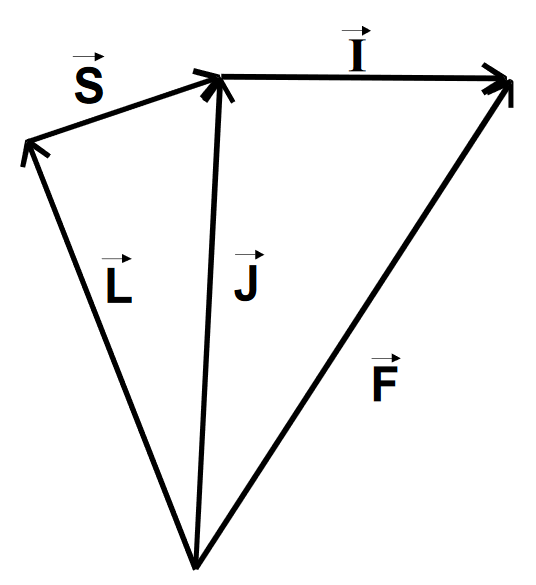
\includegraphics{./Kopplung.PNG}
  \caption{Schematische Darstellung der Zusammensetzung des Gesamtdrehimpulses $\vec{\text{F}}$\cite{Anleitung}.}
  \label{fig:F}
\end{figure}
Über die Quantenzahl F mit $|I-J|<\text{F}<I+J$ lässt sich das magnetische Moment nun durch
\begin{equation}
  \mu_F = \mu_B \text{g}_\text{F} \sqrt{F(F+1)}
  \label{eqn:mu_F}
\end{equation}
berechnen, wobei $\mu_B$ das Bohrsche Magneton und $\text{g}_\text{F}$  den sogenannten Landé-Faktor bezeichnet.
Dieses Moment sorgt dafür, dass bei einem äußeren Magnetfeld $B$ die Energieniveaus der durch den Kernspin hervorgerufenen Hyperfeinstruktur in $2\text{F}-1$ Zeeman-Niveaus aufgespalten werden. Diese Niveaus werden durch die magnetische Quantenzahl $-\text{F}<\text{m}_\text{F}<\text{F}$ beschrieben, welche aus der Eigenwertgleichung zur z-Komponente des Drehimpulses resultiert.\\
Für die Energiedifferenz zwischen benachbarten Zeeman-Niveaus gilt
\begin{equation}
  U_{Z}=\text{g}_\text{F}\mu_B B
  \label{eqn:U}
\end{equation}
Eine schematische Darstellung dieser Aufspaltung ist in Abb. \ref{fig:Zeeman} für ein Alkali-Atom mit $\mathbf{I}= \frac{3}{2}$ gegeben.
\begin{figure}[H]
  \centering
  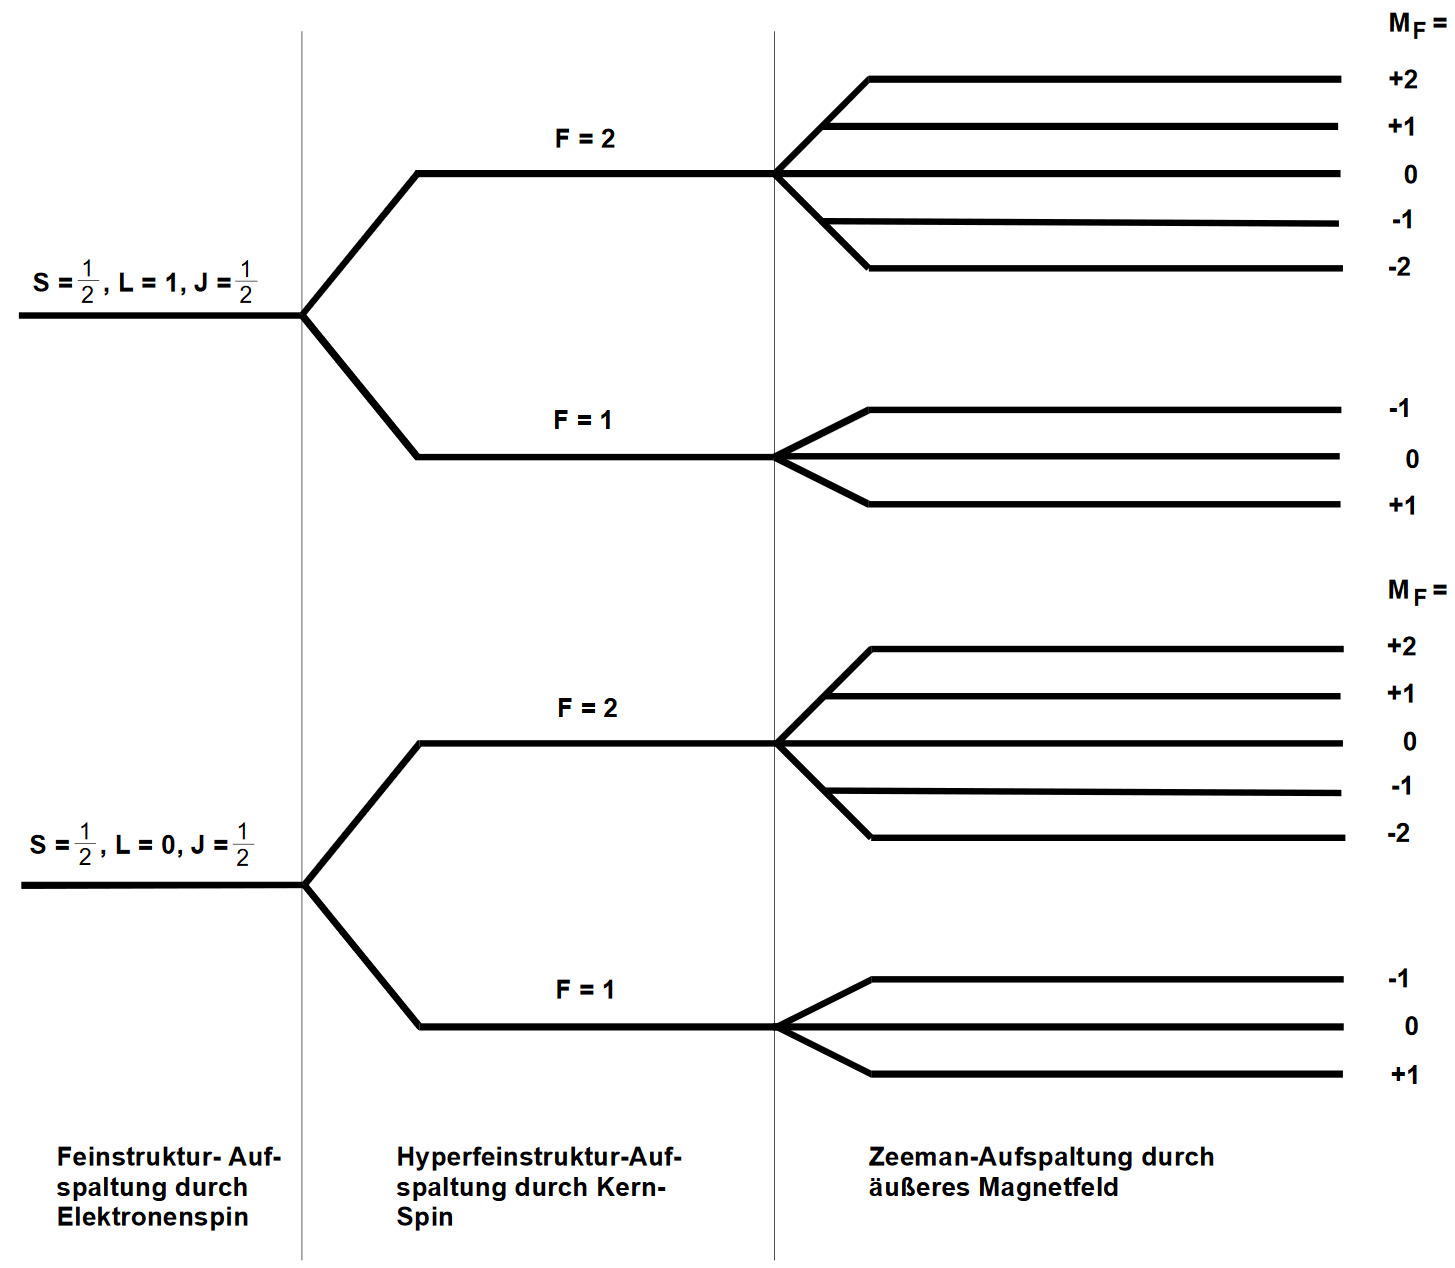
\includegraphics[width=0.9\textwidth]{./Niveaus.PNG}
  \caption{Nichtmaßstabsgetreue Darstellung der Feinstruktur-, Hyperfeinstruktur sowie Zeeman-Aufspaltung im Falle eines Alkali-Atoms mit Kernspin $\mathbf{I}= \frac{3}{2}$\cite{Anleitung}.}
  \label{fig:Zeeman}
\end{figure}
$\text{g}_\text{F}$ lässt sich mit einigen Vorüberlegungen aus den Drehimpulsquantenzahlen sowie dem kernspinfreien Landé-Faktor $\text{g}_\text{J}$ durch
\begin{equation}
  \text{g}_\text{F} \approx  \text{g}_\text{J} \frac{\text{F}\left(\text{F}+1\right)+\text{J}\left(\text{J}+1\right)-\mathbf{I}\left(\mathbf{I}+1\right)}{2\text{F}\left(\text{F}+1\right)}
  \label{eqn:gf}
\end{equation}
berechnen.
Für $\text{g}_\text{J}$ gilt hierbei
\begin{equation}
  \text{g}_\text{J} = \frac{(1+\text{g}_\text{s})\text{J}\left(\text{J}+1\right)+(1-\text{g}_\text{s})\left(\text{S}\left(\text{S}+1\right)-\text{L}\left(\text{L}+1\right)\right)}{2\text{J}\left(\text{J}+1\right)}.
  \label{eqn:gj}
\end{equation}
$\text{g}_\text{s}\approx 2,0023$ bezeichnet den Landéfaktor des freien Elektrons.\\

\subsection{Optisches Pumpen}
Das Prinzip des optischen Pumpens stützt sich vor allem darauf, dass für optisch induzierte Niveauübergänge bestimmte, von der Polarisation abhängige Auswahlregeln gelten. So gilt für linear polarisiertes Licht die Auswahlregel $\Delta m = 0$ und für rechts- bzw. links zirkularpolarisiertes Licht $\Delta m = \pm 1$. Durch diese Auswahlregeln gelingt es bestimmte Niveaus in einem Atom mit Elektronen aus energetisch niedrigeren Niveaus zu bevölkern und letztere dadurch beinahe vollständig zu leeren.\\
Strahlt man beispielsweise nur das Rubidium-D1-Licht aus einer Spektrallampe ($\lambda=\SI{795}{\nano\meter}$) auf eine Rubidiumprobe, so sind im Rubidium alle Anregungsübergänge zwischen dem $^2{S}_{1/2}$- und dem $^2{P}_{1/2}$-Zustand möglich (Vgl. Abbildung \ref{fig:Zeeman}). Wählt man nun rechtszirkular polarisiertes Licht, so muss für jede Anregung $\Delta m_{\text{F}}=+1$ gelten. Dies bedeutet, dass Elektronen, welche sich im $^2{S}_{1/2}$-Zustand mit $\text{F}=2$, $m_{\text{F}}= +2$ befinden nicht anregen lassen, da es keinen $^2{P}_{1/2}$-Zustand mit $m_{\text{F}}=+3$ gibt. Alle übrigen $^2{S}_{1/2}$
Elektronen werden angeregt, emittieren ein Photon und kehren in einen beliebigen $^2{S}_{1/2}$-Zustand zurück. Zwischen benachbarten Zeeman-Niveaus sind spontane Photonenemissionen sehr selten, weshalb sich das $\text{F}=2$, $m_{\text{F}}=+2$ Niveau des $^2{ S}_{1/2}$-Zustandes über die Zeit mit Elektronen füllt.
Die Elektronen können den Zustand dann nur durch sogenannte \textit{induzierte Emission} verlassen. Bei dieser wird durch Einstrahlung eines Photons ein Übergang in einen energetisch niedrigeren Zustand induziert. Die Energie des eingestrahlten Photons muss dabei gleich dem Betrag der Energiedifferenz des Übergangs sein. Durch Einstrahlung dieses Photons wird ein zweites Photon mit gleicher Polarisation und Energie $h\nu = U_{Z}$ emittiert. Diese Energie entspricht dann genau der zu vermessenden Differenz zwischen den beteiligten Energieniveaus.\\
\\
Die Vermessung der Energieniveaus erfolgt in diesem Versuch anhand der Aufnahme der Transparenzkurve eines optisch gepumpten, aus den Rubidium Isotopen zusammen gesetzten Gases. Eine direkte Messung der induziert emittierten Photonen ist aufgrund der quantenmechanischen Unschärfe und der Dopplerverbreitung der Spektrallinien nicht realisierbar.
In Abbildung \ref{fig:transzeit} ist die Änderung der Transparenz mit der Zeit während des Pumpvorgangs zu sehen. Es lässt sich erkennen dass die Probe sich aufgrund der durch das Pumpen enstehenden Besetzungsinversion asymptotisch der vollständigen Transparenz annähert.\\
\begin{figure}[H]
  \centering
  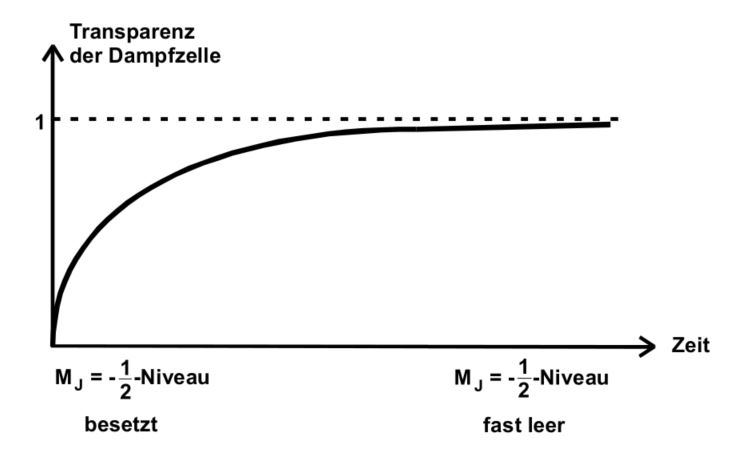
\includegraphics[width=0.6\textwidth]{plots/transzeit.JPG}
  \caption{Transparenz des Gases in Abhängigkeit von der Zeit\cite{Anleitung}.}
  \label{fig:transzeit}
\end{figure}
Die Übergangswahrscheinlichkeit eines Elektrons durch spontane Emission ist aufgrund des plankschen Strahlungsgesetzes proportional zu $\nu^3$. Da die Energiedifferenz der Zeeman-Niveaus aber sehr klein ist und somit nach $E=h\nu$ die Frequenz ebenfalls, dominiert der induzierte Emissionsprozess bei einem Zeeman-Übergang. Spontane Emission wird dagegen relevanter wenn die Energiedifferenzen höher sind wie zum Beispiel bei einem Übergang zwischen Feinstrukturniveaus. Mithilfe der induzierten Emission, lassen sich die Abstände der Zeeman-Niveaus wie folgt vermessen.\\
Zunächst legt man zusätzlich zu dem Magnetfeld, welches die Zeeman-Aufspaltung bewirkt ein frequenzvariables Hochfrequenzfeld (kurz RF-Feld) an. Anschließend wird das Zeeman-Magnetfeld  verfahren.
Da bei Null keine Zeeman-Aufspaltung existiert, findet auch kein optischer Pumpvorgang statt und die Transparenz der Probe ist gering.
Die Energiedifferenz zwischen den Zeeman-Niveaus steigt mit zunehmendem Magnetfeld gemäß
\begin{equation}
  h\nu = g_J \mu_B B \Delta M_J
\end{equation}
an und die Probe wird zunehmend intransparent. \\
Erreicht das Magnetfeld den Wert
\begin{equation}
  B_m = \frac{4\pi m_0}{e_0 g_J}\nu
\end{equation}
so entspricht die Größe der Zeeman-Aufspaltung genau der Energie des Feldes der RF-Spule und es setzt induzierte Emission ein. Dadurch verringert sich die Besetzungsinversion und die Transparenz der Probe sinkt. Dieser Vorgang wird als Resonanz bezeichnet.\\
\begin{figure}[H]
  \centering
  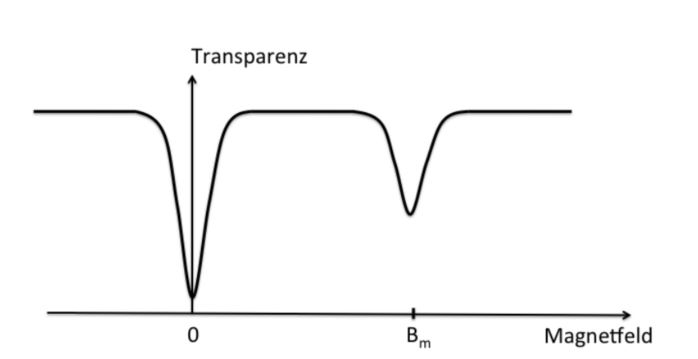
\includegraphics[width=0.6\textwidth]{plots/transfeld.JPG}
  \caption{Transparenzkurve in Abhängigkeit der Feldstärke des Zeeman-Magnetfeldes\cite{Anleitung}.}
  \label{fig:transfeld}
\end{figure}
Aus den Peakpositionen $B_m$ in der Transparenzkurve (Abbildung \ref{fig:transfeld}) und der gegebenen Frequenz $\nu$ an der RF-Spule lässt sich dann die Energiedifferenz ermitteln.
